\documentclass{beamer}
\usepackage[english]{babel}
\usepackage{calc}
\usepackage[absolute,overlay]{textpos}
\mode<presentation>{\usetheme{tud}}
%\usepackage{subcaption}

\usepackage{tikz}
\usetikzlibrary{decorations.markings}
\usetikzlibrary{shapes,snakes}
\usetikzlibrary{shapes.geometric}
\usetikzlibrary{fit}					
\usetikzlibrary{backgrounds}
\usetikzlibrary{positioning}
\usepackage{pgffor}
\usepackage{amsmath,amssymb}
\usepackage{color}



\usepackage{pifont}
\usepackage{pgfplots}

\tikzstyle{every picture}+=[remember picture]
\tikzstyle{na} = [baseline=-.5ex]


\title[]{MPM Project: Problem Description}
%\institute[]{}
\author[]{Roel Tielen, Lisa Wobbes}
\date[\today]{\today}

\definecolor{blueM}{rgb}{0.4, 0.6, 0.8}

\begin{document}
%titel----------------------------------------------------------------------------------------------------------------------------------------------------------------
{
%\usebackgroundtemplate{\includegraphics[width=\paperwidth,height=\paperheight]{logos}}%
%\setbeamertemplate{footline}{\usebeamertemplate*{minimal footline}}
\frame{\titlepage}
}

%outline------------------------------------------------------------------------------------------------------------------------------------------------------------
\begin{frame}{Outline}
\begin{itemize}
\item Oedometer problem
\item Observations with 1 PPC
\end{itemize}
\end{frame}


%------------------------------------------------------------------------------------------------------------------
\begin{frame}{Oedometer problem}
\definecolor{soil}{cmyk}{0,0.2,0.6,0.2}
\definecolor{darkred}{cmyk}{0,0.9,0.9,0.2}
\tikzset{
mystyle1/.style={
  rectangle,
  inner sep=0.05pt,
  text width=1mm,
  fill=black
  }
}

\tikzset{
mystyle2/.style={
  circle,
  inner sep=0.1pt,
  text width=2mm,
  fill=red!80
  }
}
\begin{figure}[h]
\centering
\begin{tikzpicture}
 %structure
 \draw[fill=black] (0.4,2.2) rectangle (2.6,-1.1);
 \draw[fill=soil] (0.5,2) rectangle (2.5,-1);
 \draw[fill=black!25] (0.5,2) rectangle (2.5,2.35);
 \draw (1.5, 0.5) node {soil};
 %coordinates
 \draw (3.2,2) node {$y$ = 1};
 \draw (3.2,-1) node {$y$ = 0};
 %load
 \draw[->, ultra thick,darkred] (0.7,3) -- (0.7,2.35);
 \draw[->, ultra thick,darkred] (1.5,3) -- (1.5,2.35);
 \draw[->, ultra thick,darkred] (2.3,3) -- (2.3,2.35);
 \draw (1.55,3.3) node {$p_0$};
%coordinate
\draw[->, thick] (-1,-1)--(-1,0);
\draw (-1, 0.3) node {$y$};

\draw (1.7,-2) node {schematic representation};

\end{tikzpicture}
\end{figure}
\end{frame}

%------------------------------------------------------------------------------------------------------------------
\begin{frame}{Oedometer: model}
\begin{align}\nonumber
 &\rho \frac{\partial \hat{v}}{\partial t} = \frac{\partial \hat{\sigma}}{\partial y} - \rho g, \\ \nonumber
 &\frac{\partial \hat{\sigma}}{\partial t} = E \frac{\partial \varepsilon}{\partial t}.
\end{align}
Boundary conditions: 
\begin{align} \nonumber
 &\hat{v}(0,t)  = 0,\\ \nonumber
 &\hat{\sigma}(H,t)  = -p_0.
\end{align}
Initial conditions:
\begin{align} \nonumber
 \hat{v}(y,0)&=0,\\ \nonumber
 \hat{\sigma}(y,0)&=0.
\end{align}
\end{frame}

%------------------------------------------------------------------------------------------------------------------
\begin{frame}{Oedometer: model}
\begin{equation}\nonumber
\frac{\partial^2 \hat{u}}{\partial t^2} = \frac{E}{\rho} \frac{\partial^2 u}{\partial y^2} -  g.
\end{equation}
Boundary conditions: 
\begin{align} \nonumber
 &u(0,t)  = 0,\\ \nonumber
 &\frac{\partial u}{\partial y}(H,t)  = -p_0/E.
\end{align}
Initial conditions:
\begin{align} \nonumber
& u(y,0)=0,\\ \nonumber
& \frac{\partial u}{\partial t}(y,0)=0.
\end{align}
\end{frame}

%------------------------------------------------------------------------------------------------------------------
\begin{frame}{Oedometer: discretization}
\definecolor{soil}{cmyk}{0,0.2,0.6,0.2}
\definecolor{darkred}{cmyk}{0,0.9,0.9,0.2}
\tikzset{
mystyle1/.style={
  rectangle,
  inner sep=0.05pt,
  text width=1mm,
  fill=black
  }
}

\tikzset{
mystyle2/.style={
  circle,
  inner sep=0.1pt,
  text width=2mm,
  fill=red!80
  }
}
\begin{figure}[h]
\centering
\begin{tikzpicture}
 %structure
 \draw[fill=black] (0.4,2.2) rectangle (2.6,-1.1);
 \draw[fill=soil] (0.5,2) rectangle (2.5,-1);
 \draw[fill=black!25] (0.5,2) rectangle (2.5,2.35);
 \draw (1.5, 0.5) node {soil};
 %coordinates
 \draw (3.2,2) node {$y$ = 1};
 \draw (3.2,-1) node {$y$ = 0};
 %load
 \draw[->, ultra thick,darkred] (0.7,3) -- (0.7,2.35);
 \draw[->, ultra thick,darkred] (1.5,3) -- (1.5,2.35);
 \draw[->, ultra thick,darkred] (2.3,3) -- (2.3,2.35);
 \draw (1.55,3.3) node {$p_0$};
%coordinate
\draw[->, thick] (-1,-1)--(-1,0);
\draw (-1, 0.3) node {$y$};

\draw (1.7,-2) node {schematic representation};

%discretization
\draw[-, very thick, soil] (6.2,-1)--(6.2,2);
\foreach \y in {0, ..., 3} {
      \node at (6.2,\y-1) [mystyle1] {};
    }
\foreach \y in {0, ..., 2} {
	\node at (6.2, \y-0.5) [mystyle2] {};
    }

\draw (6.2,-2) node {discretization};

\end{tikzpicture}
\end{figure}
\end{frame}


%-------------------------------------------------------------------------------------------------------------------
\begin{frame}{Oedometer: results}
\begin{overlayarea}{\textwidth}{6cm}
\begin{center}
\only<1>{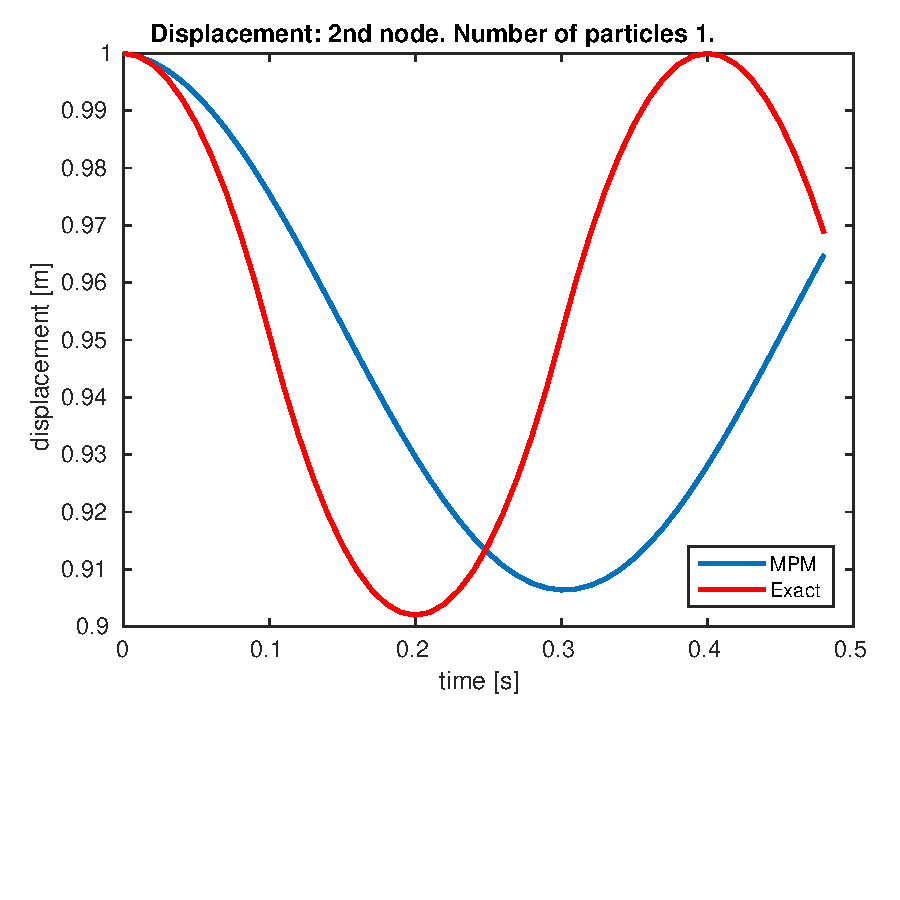
\includegraphics[scale=0.55]{images/6m_2nd_node1}
%\captionof{figure}{Error on the fine grid before smoothing.}%
%\only<1>{\includegraphics[scale=0.4]{no_smoothing_no_restriction}%
}
\only<2>{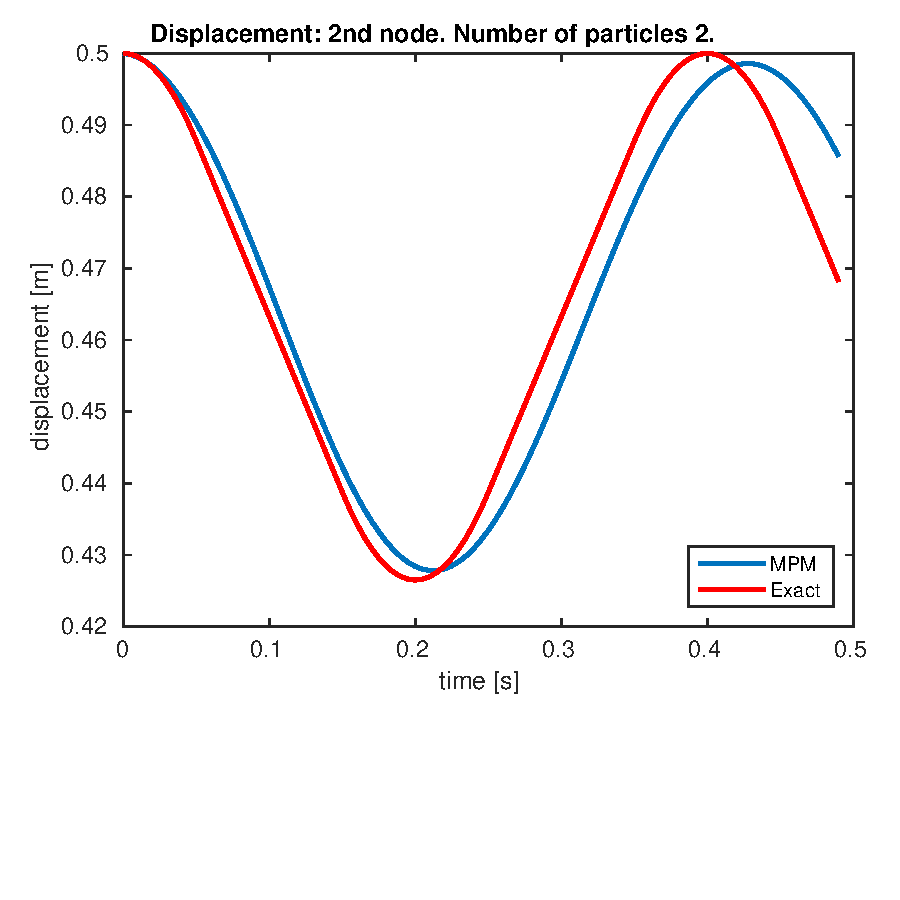
\includegraphics[scale=0.55]{images/6m_2nd_node2}%
}
\only<3>{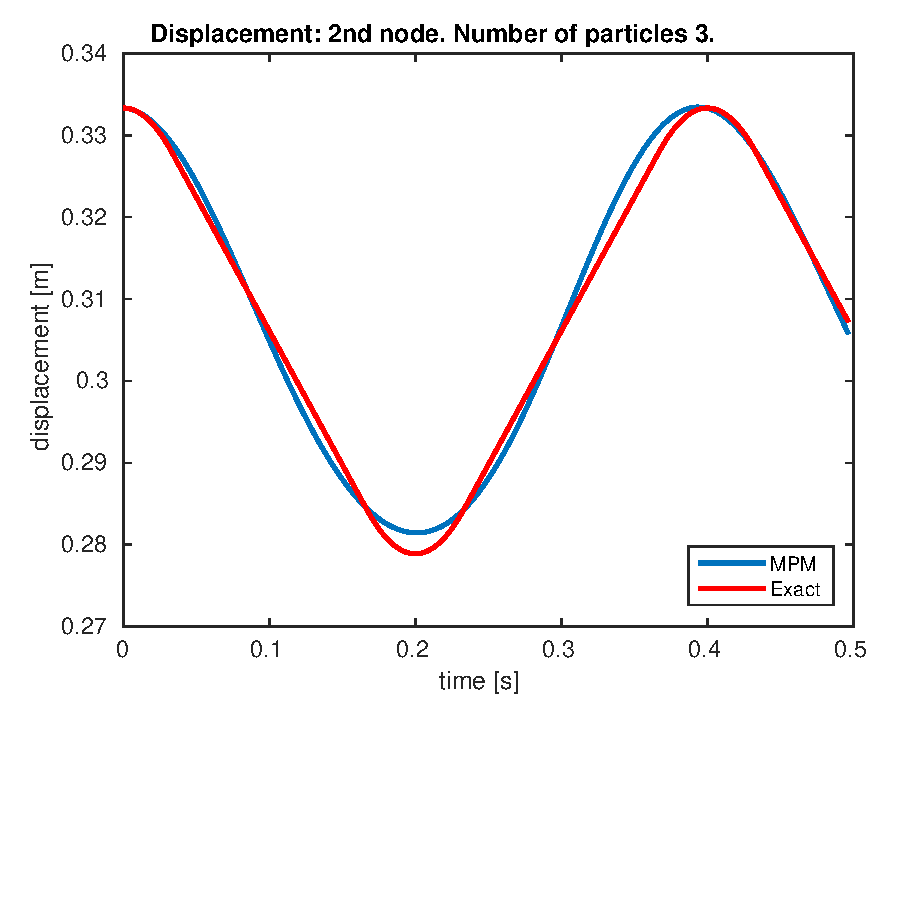
\includegraphics[scale=0.55]{images/6m_2nd_node3}%
}
\only<4>{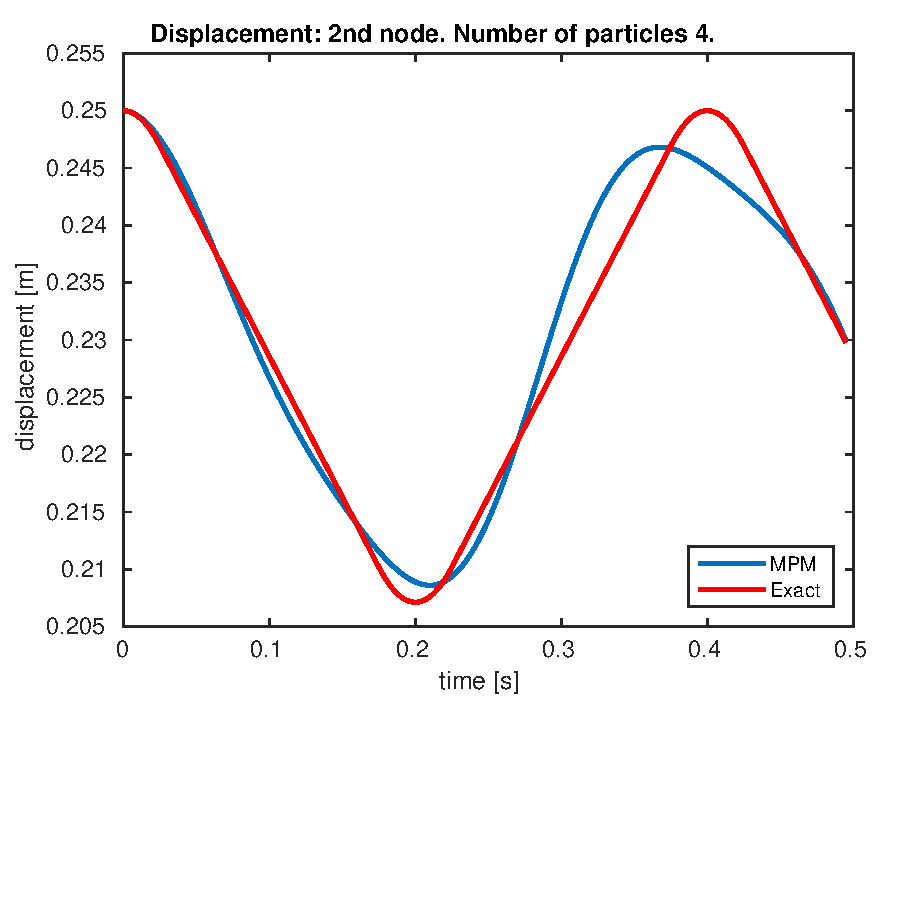
\includegraphics[scale=0.55]{images/6m_2nd_node4}%
}
\only<5>{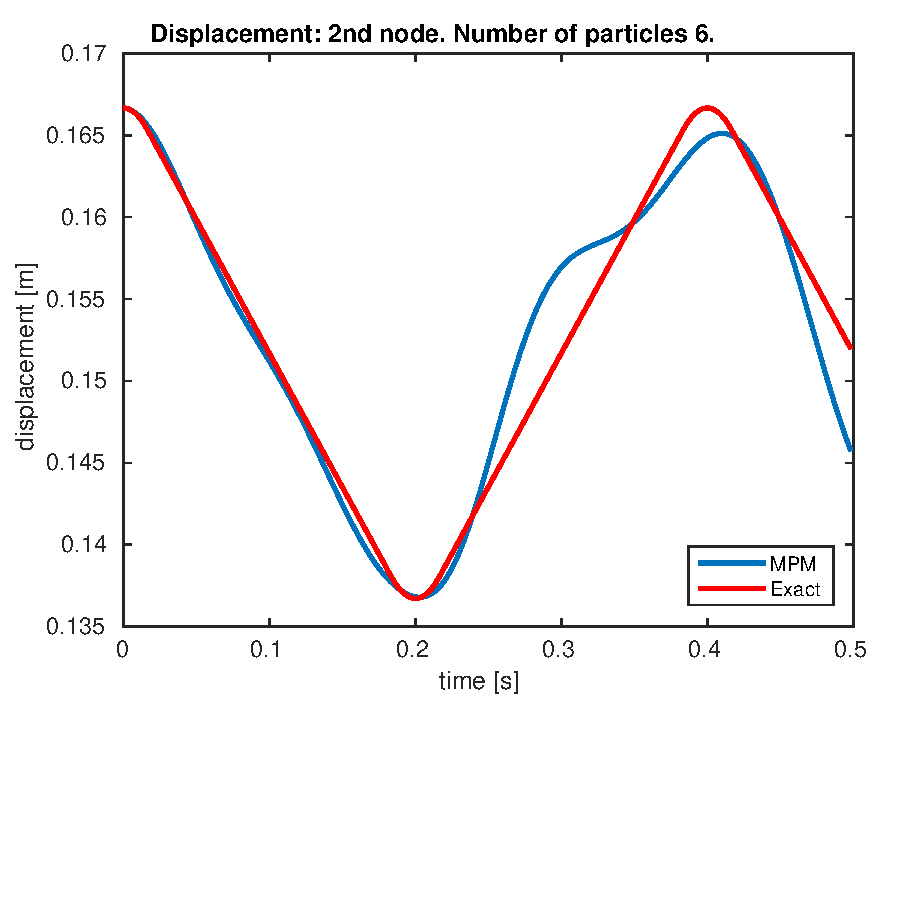
\includegraphics[scale=0.55]{images/6m_2nd_node6}%
}
\only<6>{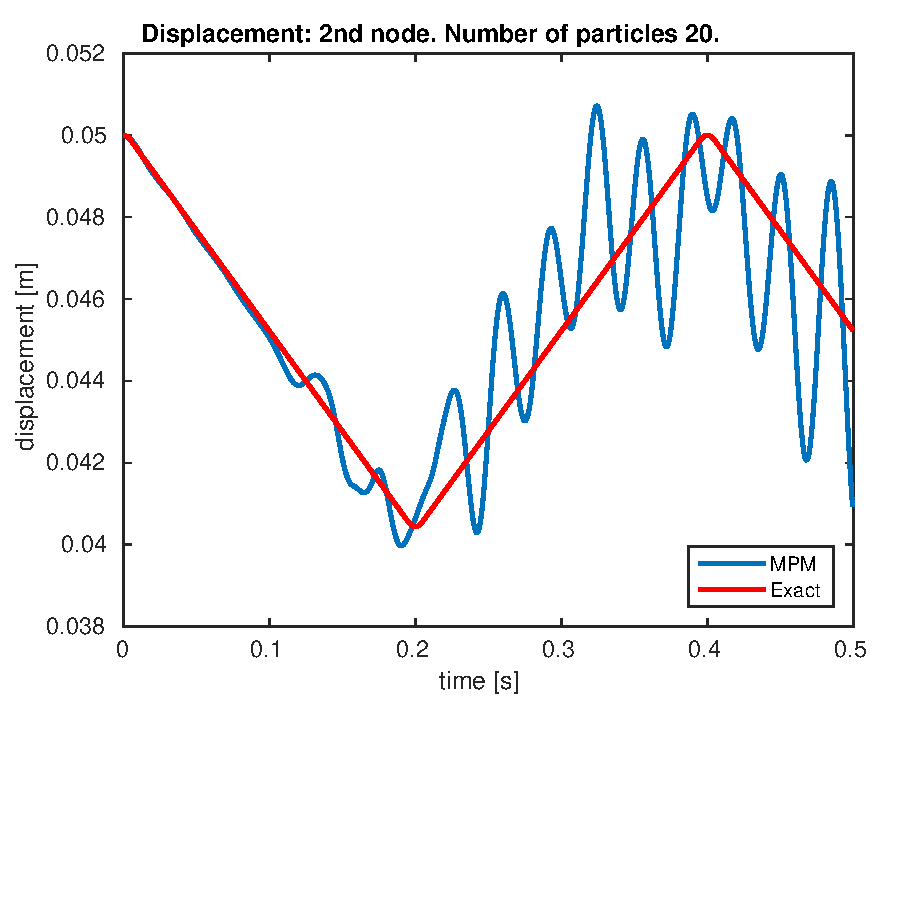
\includegraphics[scale=0.55]{images/6m_2nd_node20}%
}
\end{center}
\end{overlayarea}
\end{frame}

%-------------------------------------------------------------------------------------------------------------------
\begin{frame}{Observations}
\begin{itemize}
\item Unexpected computational artifacts due to grid crossing / appearance of empty elements.
\item Convergence only for very low number of grid nodes.
\end{itemize}


Similar observations by Bardenhagen et al.\footnote{S.~G. Bardenhagen, E.~M. Kober. \em{The generalized interpolation material point method}. Comput Model Engrg Sci, 5 (2004), pp. 477-495.} and Steffen et al.\footnote{M. Steffen, R. M. Kirby, M. Berzins. \em{Analysis and reduction of quadrature errors in the material point method (MPM)}. Int. J. Numer. Methods. Engrg, 76 (2008), pp. 922-948.}\\
Further research is required.
\end{frame}






\end{document}
\grid
